\documentclass[12pt,a4paper]{article}
\usepackage[utf8]{inputenc}
\usepackage[spanish]{babel}
\usepackage{graphicx}
\author{Prodezzargenta}
\title{Li'monero}
\begin{document}
\maketitle

\begin{abstract}
Primera marca de código abierto de un licor a base de limón para ser ofrecida a los usuarios de Monero.
\end{abstract}

\tableofcontents

\section{Introducción}
\textit{Li'monero} es una marca de código abierto de licor de limón. El objetivo de esta marca es proporcionar tanto un producto de bajo coste de fabricación, como también un modelo de emprendimiento de bajo costo para incentivar el uso de Monero como bien de intercambio en el mercado paralelo (y alejarse, así, de su utilización como activo financiero para realizar \textit{forex trading}\footnote{Es decir, el \textit{trading} de Monero, en las diferentes casas de cambio públicas, para su compraventa; con el fin de obtener ganancias en dinero \textit{fiat} (entiéndase esto como dólares o euros, en el mercado occidental).}).

\subsection{Nombre}
El nombre \textit{Li'monero} es un juego de palabras que se desglosa de la siguiente manera: 

\begin{itemize}
\item \textbf{Limonero}: árbol frutal perenne.
\item \textbf{Li'mo}: un término \textit{informal}, creado por el autor en idioma inglés, para referirse al \textit{limón}.
\item \textbf{Li'mone}: \textit{limón} en idioma italiano (con un apóstrofe en la primera sílaba)\footnote{Esta referencia se debe a que el licor hace referencia al \textit{limoncello}.}.
\item \textbf{Li'mone + nero («Limón negro»)}: en referencia a una bebida alcohólica creada con limones para ser vendida en el mercado «negro»\footnote{Aunque este término tenga una connotación negativa, se hace referencia al mercado \textit{paralelo}.}.
\item \textbf{Li'mo + monero («Limón [de] Monero»)}: marca creada para que los usuarios de Monero puedan comprarlo, (o crearlo y venderlo), para ofrecer un producto más en el mercado; y utilizar Monero como dinero usuario-a-usuario (\textit{P2P cash}).
\end{itemize}

\subsection{Resumen}
Consiste en una bebida a base de limón, alcohol y almíbar. Se ofrecen dos recetas: una etiqueta «estándar» y una etiqueta «\textit{premium}». La diferencia radica en que la primera está hecha a base de vodka; mientras que la segunda está hecha a base de alcohol alimenticio.

Si bien los procesos para la preparación consiste en largos períodos de tiempo, la bebida no requiere de ningún tipo de especialización de ninguna área. Sólo se requiere de dos procesos importantes: primero, la correcta limpieza de los frascos donde se almacenará la bebida (tanto en los recipientes donde se hará como en las botellas donde se verterá el producto terminado); y, segundo, el almacenamiento del preparado en lugares frescos y oscuros, correctamente sellado para que no tenga contacto con el aire.

Los pasos a seguir son los siguientes:

\begin{enumerate}
\item Pelar la cáscara de limones en trozos pequeños. Cuidado con pelar la «piel blanca» del limón: esto empeorará el sabor. Colocar todos los trozos pequeños en el frasco de vidrio.
\item Colocar el contenido de alcohol.
\item Sellar el frasco con film adherente para prevenir que el aire esté en contacto con el alcohol.
\item Almacenar el frasco en un lugar fresco y oscuro.
\item Sacudir el frasco todos los días durante 30 días..
\item En una cacerola con agua bebible y azúcar, batir constantemente hasta llegar al punto de ebullición.
\item Dejar que el almíbar se enfríe a temperatura ambiente; verter el contenido frío en el frasco y sellarlo nuevamente.
\item Sacudir, una vez más, el frasco todos los días durante 30 días..
\item Tomar las botellas de vidrio esterilizadas y, con el embudo con algodón, filtrar la preparación. Si es necesario, filtrarlo nuevamente. La bebida no debe contener ningún tipo de residuo o material sólido.
\item Almacenar las botellas en un refrigerador.
\end{enumerate}

\section{Certificado}
En la cuenta de GitHub del autor se adjuntará la llave pública GPG en un archivo \texttt{.asc}. Éste archivo está firmado por el autor de la marca, y encriptado con la llave privada con una clave GPG para certificar que la receta y los demás archivos están \textit{legitimados} por el autor.

Este procedimiento sirve para ofrecer un grado más de seguridad y autenticidad tanto para el cliente que desea comprar un producto de la marca, como también del fabricante que desee producirlo. Para verificar esta autenticidad, el usuario deberá realizar los siguientes pasos:

\begin{enumerate}
\item Descargar el archivo \texttt{.asc} que contiene la llave pública GPG.
\item Descodificar el archivo que contiene todos los datos sobre la fabricación del producto utilizando la llave pública GPG\footnote{Este procedimiento debe hacerse cuando las dos partes han intercambiado sus respectivas llaves privadas, y el archivo de texto o mensaje está encriptado. Si no lo está, avanzar al siguiente paso.}.
\item Verificar que la firma adjuntada es válida con la llave pública GPG\footnote{Aunque este proceso podría parecer innecesario cuando las dos partes han intercambiado sus respectivas llaves públicas, una cosa es encriptar/descifrar un mensaje, y otra cosa es verificar el \textit{contenido} del mismo mensaje. Este procedimiento debe ser realizado para asegurar la autenticidad.}.
\end{enumerate}

\subsection{Contenido}
En este archivo encriptado, aparecerán los siguientes datos:

\begin{itemize}
\item \textbf{INFORMACIÓN}: Información de la marca de código abierto.
	\begin{itemize}
	\item \textbf{NOMBRE}: Nombre del autor de la marca de código abierto.
	\item \textbf{MARCA}: Nombre de la marca de código abierto.
	\item \textbf{DIRECCIÓN}: Dirección de Monero del autor de la marca.
	\item \textbf{TIPO DE COMISIÓN}: Forma en la que se estipula el pago de la comisión.
	\item \textbf{COMISIÓN}: Porcentaje de comisión según lo estipulado por el autor.
	\end{itemize}
\item \textbf{HASH}: Listado de sumas \textit{hash} de los archivos adjuntados en GitHub.
\item \textbf{MATERIALES:} Listado de materiales necesarios para todo el proceso de fabricación del producto.
\item \textbf{PROCEDIMIENTO:} Proceso de trabajo para la fabricación del producto.
\item \textbf{NOTA:} Cualquier observación o comentario realizado por el autor.
\end{itemize}

\section{Imágenes}

\subsection{Logo principal}

\begin{center}
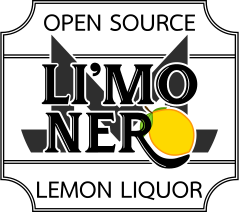
\includegraphics[width=1\textwidth]{img/logo.pdf}
\end{center}

\subsection{Etiquetas}
\begin{center}
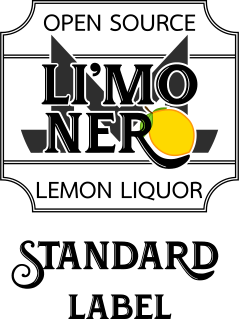
\includegraphics[width=1\textwidth]{img/std-label.pdf}
\end{center}

\begin{center}
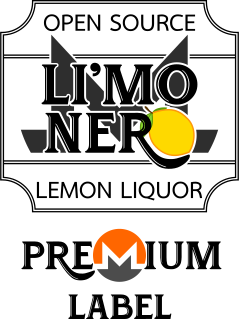
\includegraphics[width=1\textwidth]{img/prm-label.pdf}
\end{center}

\end{document}